% Inside the direction and separation node, for one 128 ms chunk (doa_separation_node/node.py, model/streaming_net.py,
% model/tracker.py). Upper lane: separated voices; lower lane: tracks. The tracker's slot-to-track map gives each voice its track id.
% Orange: the point where the network's spectra become audio again.
\documentclass[border=1.5pt]{standalone}
% Shared look of the figures in docs/. Text 8 pt, Times.
% Colors: cInk for this device's code and data, cFace (grey fill) for hardware, cCal for the one point each figure is about.
\usepackage[T1]{fontenc}
\usepackage{times}
\usepackage{amsmath,amssymb}
\usepackage{xcolor}
\usepackage{tikz}
\usepackage{pgfplots,pgfplotstable}
\pgfplotsset{compat=1.18}
\usetikzlibrary{arrows.meta,positioning,calc}
\usepgfplotslibrary{groupplots}

\definecolor{cCal}{HTML}{D55E00}
\definecolor{cInk}{HTML}{1F2933}
\definecolor{cMuted}{HTML}{6B7280}
\definecolor{cGrid}{HTML}{E3E6EA}
\color{cInk}

\newcommand{\figfont}{\fontsize{8}{9.5}\selectfont}
\newcommand{\figsmall}{\fontsize{8}{9.5}\selectfont}

\pgfplotsset{
  spl/.style={
    width=44mm, height=36mm, scale only axis=false,
    axis line style={cMuted, line width=0.5pt},
    tick style={cMuted, line width=0.5pt}, tick align=outside,
    tick label style={font=\figsmall, text=cInk},
    label style={font=\figfont, text=cInk},
    legend style={font=\figsmall, draw=none, fill=none, text=cInk, inner sep=0pt},
    legend cell align=left,
    grid=major, major grid style={cGrid, line width=0.4pt},
    axis lines*=left, clip mode=individual,
    every axis plot/.append style={line width=0.9pt},
  },
}

\definecolor{cFace}{HTML}{E2E5E9}
\begin{document}
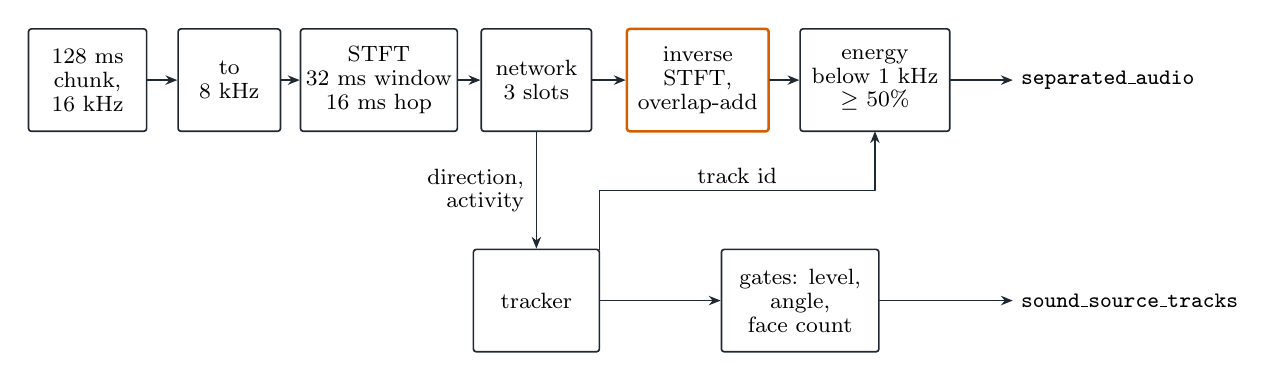
\begin{tikzpicture}[x=1mm, y=1mm, font=\figfont, line join=round, line cap=round,
  own/.style={draw=cInk, line width=0.6pt, rounded corners=1pt, align=center, inner xsep=0.7mm, inner ysep=0.8mm, fill=white, minimum height=13mm},
  flow/.style={-{Stealth[length=1.5mm, width=1.2mm]}, line width=0.6pt, draw=cInk},
  topic/.style={font=\ttfamily\bfseries\figsmall, inner sep=0pt},
  card/.style={align=left, inner sep=0pt}]

\node[own, minimum width=15mm] (chunk) at (7.5,40) {128 ms\\[-0.3mm]chunk,\\[-0.3mm]16 kHz};
\node[own, minimum width=13mm] (dec)   at (25.5,40) {to\\[-0.3mm]8 kHz};
\node[own, minimum width=17mm] (stft)  at (44.5,40) {STFT\\[-0.3mm]32 ms window\\[-0.3mm]16 ms hop};
\node[own, minimum width=14mm] (net)   at (64.5,40) {network\\[-0.3mm]3 slots};
\node[own, minimum width=18mm, draw=cCal, line width=0.9pt] (istft) at (85,40) {inverse\\[-0.3mm]STFT,\\[-0.3mm]overlap-add};
\node[own, minimum width=19mm] (low)   at (107.5,40) {energy\\[-0.3mm]below 1 kHz\\[-0.3mm]$\geq$ 50\%};
\draw[flow] (chunk.east) -- (dec.west);
\draw[flow] (dec.east) -- (stft.west);
\draw[flow] (stft.east) -- (net.west);
\draw[flow] (net.east) -- (istft.west);
\draw[flow] (istft.east) -- (low.west);
\draw[flow] (low.east) -- (125,40);
\node[topic, anchor=west] at (126,40) {separated\_audio};

\node[own, minimum width=16mm] (trk)  at (64.5,12) {tracker};
\node[own, minimum width=20mm] (gate) at (98,12) {gates: level,\\[-0.3mm]angle,\\[-0.3mm]face count};
\draw[flow] (net.south) -- (trk.north);
\node[card, anchor=east, align=right] at (63,26) {direction,\\[-0.4mm]activity};
\draw[flow] (trk.east) -- (gate.west);
\draw[flow] (gate.east) -- (125,12);
\node[topic, anchor=west] at (126,12) {sound\_source\_tracks};
\draw[flow] (72.5,18.5) -- (72.5,26) -| (107.5,33.5);
\node[card, anchor=south, inner sep=0.8mm] at (90,26) {track id};
\end{tikzpicture}
\end{document}
